\lecture{运算符重载}{lec:chap04}
\section[运算符重载]{从函数重载到运算符重载}\label{sec:chap04-sec01}
%%%%%%%%%%%%%%%%%%%%%%%%%%%%%% 从函数重载到运算符重载 %%%%%%%%%%%%%%%%%%%%%%%%%%%%%%%%%%
\begin{frame}[t, fragile]{运算符重载}{接口的多态性}%
  \begin{spacing}{1.8}
    \begin{itemize}
    \item 使用一致接口(uniform interface)处理不同数据
    \begin{itemize} 
    \item 函数重载 
    \item 运算符重载(``\cppinttfts{+}'')
      \begin{center}
        \begin{tikzpicture}[font=\tiny, show background grid]
          \umlnote[scale=1.0, text width=0.5\textwidth](note) {
            \begin{cppttnobg}
3.14 + 0.0015 = 3.1415;
[1, 2, 3] + [4, 5, 6] = [1, 2, 3, 4, 5, 6];
[3 + 4i] + [1 + 5i] = [4 + 9i];
"coffee" + " tea" = "coffee tea";
           \end{cppttnobg}
          };
        \end{tikzpicture}
      \end{center}
    \item 虚函数(继承与派生)
    \end{itemize}  
    \end{itemize}
  \end{spacing}
\end{frame}

\begin{frame}[t, fragile]{运算符重载}{函数重载的演化}%
  \stretchon
  \begin{itemize}
  \item 函数重载
    \begin{itemize}
    \item 功能相同、数据不同(类型或个数)的同名函数
    \end{itemize}
  \item 运算符重载
    \begin{itemize}
    \item 同一个运算符作用于不同类型数据的操作
    \item 运算符$\Rightarrow$ \alert{函数名}
    \end{itemize}
  \end{itemize}
  \stretchoff
\end{frame}

\begin{frame}[t, fragile]{运算符重载}{函数重载的演化}%
  \stretchon
  \begin{itemize}
  \item 运算符重载是C++的一大亮点
    \begin{itemize}
    \item 函数调用更简洁、直观
    \item 增加程序可读性(readability)
    \end{itemize}
  \item 实际应用
    \begin{itemize}
    \item 复数操作:\cppinttfts{(a+bi)+(c+di) = (a+c) + (b+d)i}
    \item 字符串操作:\cppinttfts{string1 == string2}
    \item 向量操作:\cppinttfts{(a1, |$\cdots$|, an)*s = (a1*s, |$\cdots$|, an*s)}
    \item 矩阵乘法:\cppinttfts{M = N*K}
    \item $\cdots$
    \end{itemize}
  \end{itemize}
  \stretchoff
\end{frame}

\begin{frame}[t, fragile]{运算符重载}{实例:经纬度类}%
  \begin{spacing}{1.5}
  \begin{itemize}
  \item 位置信息:纬度(latitude)和经度(longitude)
  \item 经纬度决定地球上一个地点的精确位置    
  \end{itemize}
  \begin{center}
    \begin{boxedminipage}{0.95\linewidth}
      \footnotesize      
      \heiti{已知:}

      \parindent=2em 北京天安门:(39.907306, 116.391264)

      \parindent=0em \heiti{求:}

      \parindent=2em 西南方向偏移(-5.642159, -8.323558)后的新位置?

      \parindent=0em \heiti{解:}

      \parindent=2em \fbox{\scriptsize \colorbox{green}{39.907306 + (- 5.642159)}}\quad\fbox{\scriptsize \colorbox{green}{116.391264 + (-
        8.323558)}}

      \parindent=0em \heiti{答案:}

      \parindent=2em    (34.265147 108.067706)$\Rightarrow$  西北农林科技大学行政楼位置
    \end{boxedminipage}
  \end{center}
  \end{spacing}
\end{frame}

\begin{frame}[t, fragile]{运算符重载}{实例:经纬度类}%
  \begin{spacing}{1.8}
  \begin{itemize}
  \item 位置信息:纬度(latitude)和经度(longitude)
  \item 经纬度决定地球上一个地点的精确位置    
  \end{itemize}  
  \begin{center}
    \begin{tabular}{ccc}
      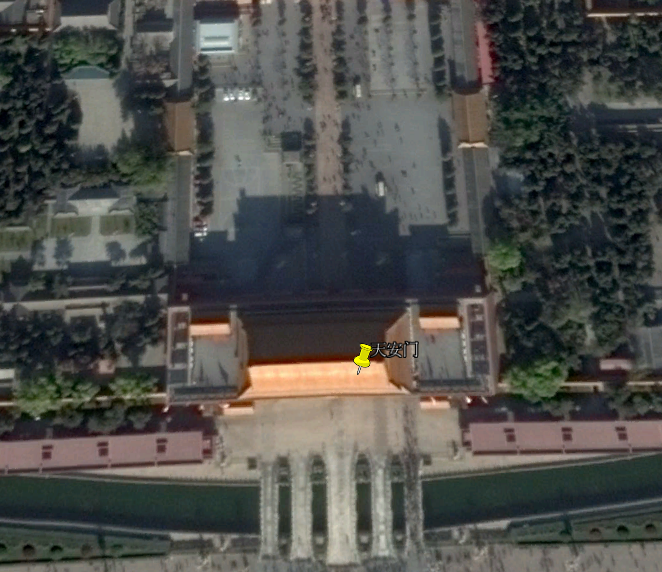
\includegraphics[align=c,width=0.4\textwidth]{chap04/01tiananmen} & $\Rightarrow$ & 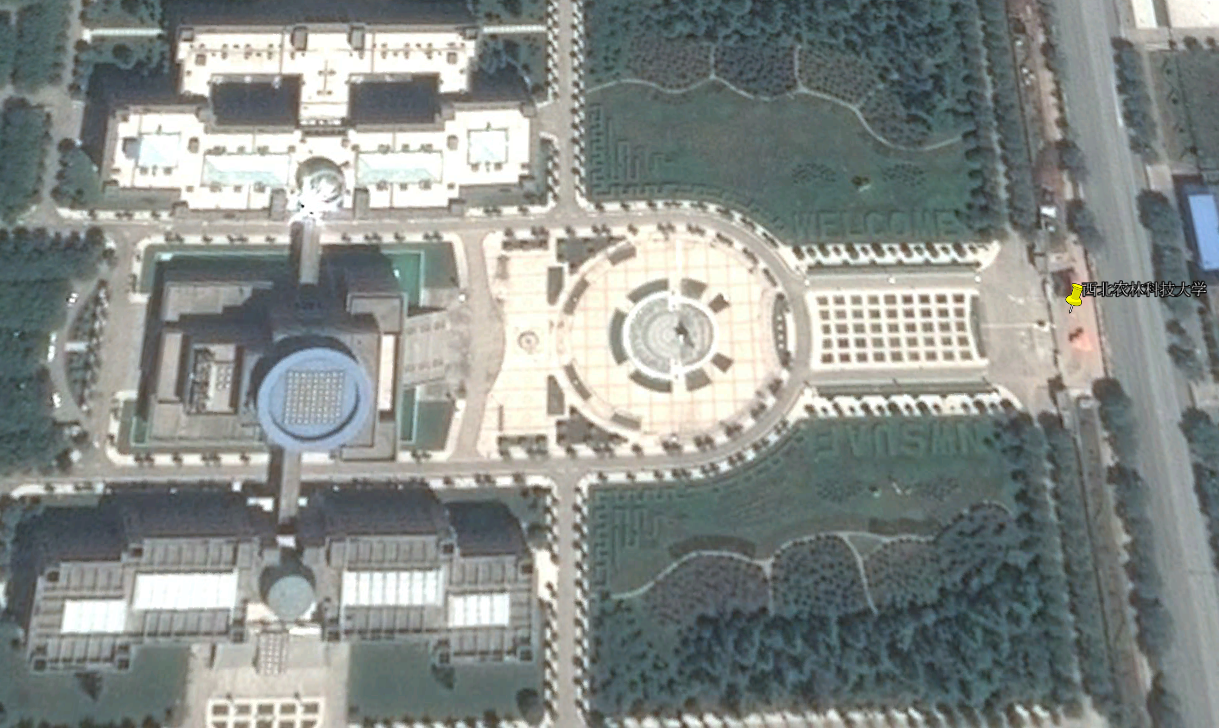
\includegraphics[align=c,width=0.4\textwidth]{chap04/02nwsuaf}
    \end{tabular}
    %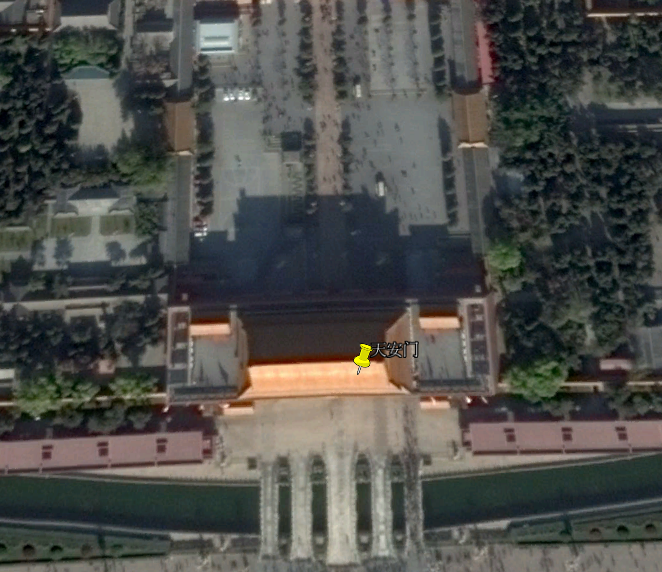
\includegraphics[width=0.45\textwidth]{chap04/01tiananmen}
    %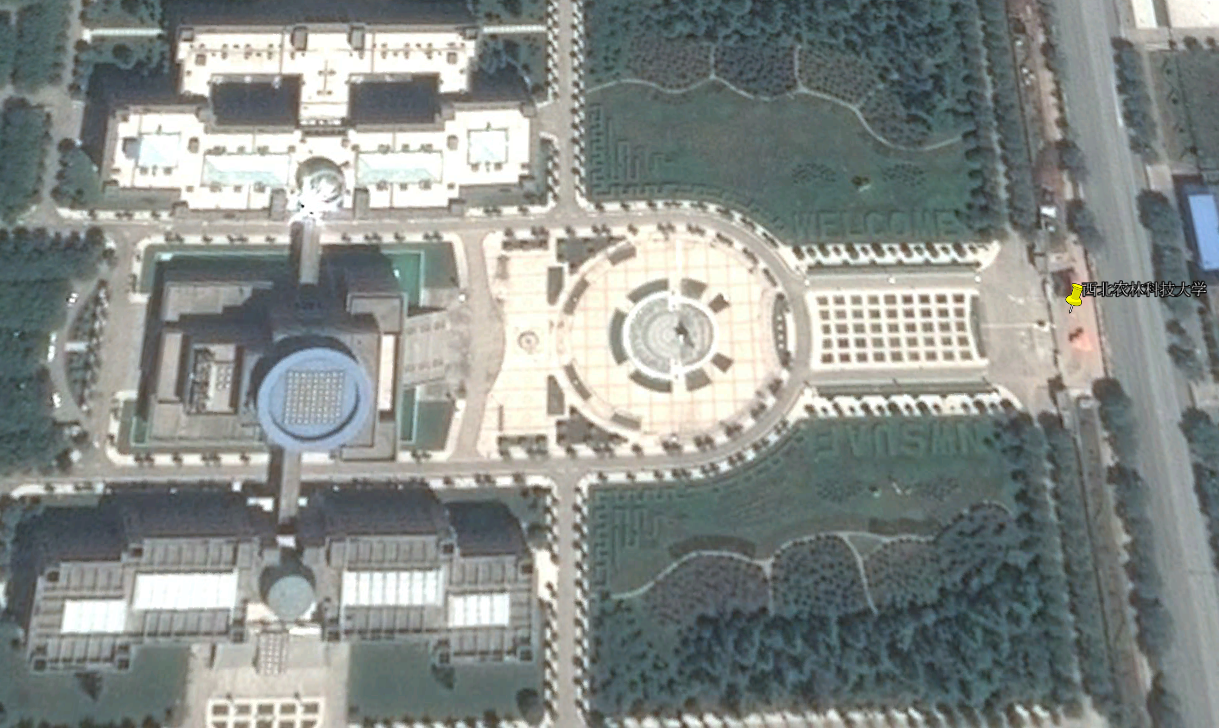
\includegraphics[width=0.45\textwidth]{chap04/02nwsuaf}
  \end{center}
  \end{spacing}
\end{frame}

\begin{frame}[ t, fragile]{运算符重载}{实例:经纬度类}%
  \begin{itemize}
  \item 位置信息:纬度(latitude)和经度(longitude)
  \item 经纬度决定地球上一个地点的精确位置    
  \end{itemize}
  \begin{center}
    \begin{tikzpicture}[font=\tiny, show background grid]
      \tikzset{
        coord/.style={coordinate}
      }          
      \umlnote[scale=0.85, text width=0.55\textwidth](code1) at (0,0) {
        \cppfilettnobg{codes/chap04/ex04-01-01-CLocation.cpp}
      };
      \umlnote[scale=0.9, text width=0.52\textwidth](code2) at ($(code1.north) + (5.0, 0.0)$) {
        \cppfilettnobg{codes/chap04/ex04-01-02-main.cpp}
      };

      % Now we place the coordinate nodes for the connectors with
      % angles, or with annotations. , coord
      \node [coord] (c1) at ($(code1) + (-1.15, -1.20)$) {};
      \node [coord] (c2) at ($(code1) + (-0.4, -1.7)$) {};
      \node [coord] (c3) at ($(code2) + (-1.5, 0.5)$) {};
      \node [coord] (c4) at ($(code2) + (-1.5, 0.12)$) {};
      \node [coord] (c5) at ($(code2) + (-2.2, -1.00)$) {};  
    

      \node [draw, fill=blue!25] (note1) at ($(code1) +(1.0, 0)$)
      {\alert{+}运算符的重载};
      \node[draw, align=center, fill=blue!25] (note2) at ($(code2) +(1.2, 1.1)$)
      {北京天安门:\\(39.907306, 116.391264)};
      \node [draw, align=center, fill=blue!25] (note3) at ($(code2) +(1.2, -1.5)$)
      {西南方向偏移:\\(-5.642159, -8.323558)};
      \node [draw, align=center, fill=blue!25] (note4) at ($(code2) +(-0.8, -2.5)$)
      {西北农林科技大学\\行政楼位置};
      
      \draw[-{Stealth[scale=1.0]},red, thick] (note1.south)--(c1);
      \draw[-{Stealth[scale=1.0]},red, thick] (note1.south)--(c2);
      \draw[-{Stealth[scale=1.0]},red, thick] (note2.west)--(c3);
      \draw[-{Stealth[scale=1.0]},red, thick] (note3.north)--(c4);
      \draw[-{Stealth[scale=1.0]},red, thick] (note4.north)--(c5);
    \end{tikzpicture}
  \end{center}
\end{frame}
%%%%%%%%%%%%%%%%%%%%%%%%%%%%%%%%%%%%%%%%%%%%%%%%%%%%%%%%%%%%%%%%%%%%%%%%%%%%%%%

\section[重载规则]{运算符重载规则}\label{sec:chap04-sec02}
%%%%%%%%%%%%%%%%%%%%%%%%%%%%%% 运算符重载规则 %%%%%%%%%%%%%%%%%%%%%%%%%%%%%%%%%%
\begin{frame}[t, fragile]{重载规则}{运算符重载规则}%
  \begin{spacing}{1.8}
  \begin{itemize}
  \item 可重载的运算符\\
    \begin{center}
      %\begin{minipage}{0.8\linewidth}
        \scriptsize
        \begin{tabular}{|c|c|c|c|c|c|c|c|c|}
          \hline
          \cppinttscr{+} & \cppinttscr{-} & \cppinttscr{*} & \cppinttscr{/} & \cppinttscr{%} & 
          \cppinttscr{^} & \cppinttscr{&} & \cppinline[fontsize=\scriptsize]{|} & \cppinttscr{~} \\

          \hline
          \cppinttscr{!} & \cppinttscr{,} & \cppinttscr{=} & \cppinttscr{<} & \cppinttscr{>} & 
          \cppinttscr{<=} & \cppinttscr{>=} & \cppinttscr{++} & \cppinttscr{--} \\

          \hline
          \cppinttscr{<<} & \cppinttscr{>>} & \cppinttscr{==} & \cppinttscr{!=} & \cppinttscr{&&} & 
          \cppinline[fontsize=\scriptsize]{||} & \cppinttscr{+=} & \cppinttscr{-=} & \cppinttscr{/=} \\

          \hline
          \cppinttscr{%=} & \cppinttscr{^=} & \cppinttscr{&=} & \cppinline[fontsize=\scriptsize]{|=} & \cppinttscr{*=} & 
          \cppinttscr{<<=} & \cppinttscr{>>=} & \cppinttscr{[]} & \cppinttscr{()} \\

          \hline
          \cppinttscr{->} & \cppinttscr{->*} & \cppinttscr{new} &
                                                               \cppinttscr{new []} & \cppinttscr{delete} & 
          \cppinttscr{delete []} &  &  & \\
          \hline
        \end{tabular}
      %\end{minipage}
    \end{center}
  \item 单目运算符和双目运算符
  \item 不可重载的运算符\\
    \begin{center}
      %\begin{minipage}{0.8\linewidth}
        \scriptsize
        \begin{tabular}{|c|c|c|c|}
          \hline
          \cppinttscr{.} & \cppinttscr{.*} & \cppinttscr{::} & \cppinttscr{?:}\\
          \hline
        \end{tabular}
      %\end{minipage}
    \end{center}
  \end{itemize}
  \end{spacing}
\end{frame}

\begin{frame}[t, fragile]{重载规则}{运算符重载规则}%
  \stretchon
  \begin{itemize}
  \item 重载规则
    \begin{itemize}
    \item 重载后运算符的优先级和结合性不变
    \item 运算符操作数的个数不能改变
    \item 不能重载C++中不支持的运算符 (@、\#、\$等)
    \item 保持运算符的语义%\\
      % \begin{tikzpicture}[font=\tiny, show background grid]
      %   \umlnote[text width=0.6\textwidth](note) at (0,0)
      %   {
      %     \begin{cppttnobg}
      %       bool operator!( const string &s1, const string &s2 )
      %       {
      %         return( strcmp( s1.c_str(), s2.c_str() ) != 0 );
      %       }
      %     \end{cppttnobg}
      %   };
      %   \node at (4.5, -1) {\Large \badmark};
      % \end{tikzpicture}
    \end{itemize}
  \end{itemize}
  \stretchoff
\end{frame}
%%%%%%%%%%%%%%%%%%%%%%%%%%%%%%%%%%%%%%%%%%%%%%%%%%%%%%%%%%%%%%%%%%%%%%%%%%%%%%%

\section[重载方式]{运算符重载方式}\label{sec:chap04-sec03}
%%%%%%%%%%%%%%%%%%%%%%%%%%%%%% 运算符重载方式 %%%%%%%%%%%%%%%%%%%%%%%%%%%%%%%%%%
\begin{frame}[t, fragile]{重载方式}{运算符重载方式}%
  \begin{spacing}{1.8}
  \begin{itemize}
  \item 重载为类的成员函数
    \begin{itemize}
    \item 定义\\
      \begin{center}
        \begin{minipage}{0.8\linewidth}
          \begin{cpptt}
|返回类型| [|类名|::]operator |运算符|(|形参表|) {}
CLocation operator+(CLocation op2);
          \end{cpptt}
        \end{minipage}
      \end{center}
    \end{itemize}
  \item 重载为类的非成员函数(\alert{一般为友员函数})
    \begin{itemize}
    \item 定义\\
      \begin{center}
        \begin{minipage}{0.8\linewidth}
          \begin{cpptt}
friend |返回类型| operator |运算符|(|形参表|) {}
          \end{cpptt}
        \end{minipage}
      \end{center}
    \end{itemize}
  \end{itemize}
  \end{spacing}
\end{frame}

\begin{frame}[t, fragile]{重载方式}{重载为类的成员函数}%
  \begin{spacing}{1.6}
  \begin{itemize}
  \item 语法:\cppinlinett{|返回类型| [|类名|::]operator |运算符|(|形参表|) {}}
    \begin{itemize}
    \item 返回类型一般是一个对象
    \item 可以省略一个形参\\
      \begin{tikzpicture}[font=\tiny, show background grid]
        \umlnote[text width=0.5\textwidth](note) at (0,0)
        {
          \begin{cppttnobg}
CLocation operator+(CLocation op2);
CLocation operator-(CLocation op2);
CLocation operator=(CLocation op2);
CLocation operator++();
          \end{cppttnobg}
        };
      \end{tikzpicture}           
    \end{itemize}
  \end{itemize}
  \begin{center}
    \begin{minipage}{0.6\linewidth}
      \tiny
      注意:用成员函数实现+运算符重载,只有一个参数!\\
      \begin{cppcode}
CLocation loc1(30,100), loc2(5,4);
loc1 = loc1 + loc2;
      \end{cppcode}
      \\ \alert{另一参数通过this指针隐式传递!}
    \end{minipage}
  \end{center}
  \end{spacing}
\end{frame}

\begin{frame}[t, fragile]{重载方式}{实例:经纬度类}%
  \begin{itemize}
  \item 重载函数定义\\
    \begin{center}
      \begin{tikzpicture}[font=\tiny, show background grid]
        \tikzset{ coord/.style={coordinate} }
        \umlnote[text width=0.52\textwidth](code1) at (0,0)
        {
          \cppfilettnobg{codes/chap04/ex04-02-01-CLocation.cpp}
        };
        \umlnote[text width=0.33\textwidth](code2) at ($(code1.north) + (4.8,0)$)
        {
          \cppfilettnobg{codes/chap04/ex04-02-02-main.cpp}
        };

        % Now we place the coordinate nodes for the connectors with
        % angles, or with annotations. , coord
        \node [coord] (c1) at ($(code1) + (-3.2, -0.95)$) {};
        \node [coord] (c2) at ($(c1) + (1.4, 0)$) {};
        \node [coord] (c3) at ($(code1) + (-3.2, -2.2)$) {};
        \node [coord] (c4) at ($(c3) + (1.4, 0)$) {};
        \node [coord] (c5) at ($(code2) + (-1.85, -0.1)$) {};
        \node [coord] (c6) at ($(code1) + (0.1, -1.2)$) {};
        \node [coord] (c7) at ($(code2) + (-1.85, -0.8)$) {};
        \node [coord] (c8) at ($(code1) + (0.8, -0.2)$) {};
        \node [coord] (c9) at ($(code2) + (-1.85, -1.0)$) {};
        \node [coord] (c10) at ($(code1) + (0.8, 1.3)$) {};

        \node [draw, fill=blue!25] (note1) at ($(code1) + (1.2, -3.2)$)
      {利用\alert{*this}指针返回运算后的对象};

        \draw[blue, thick] (c1)--(c2);
        \draw[blue, thick] (c3)--(c4);
        \draw[-{Stealth[scale=1.0]},red, thick] (c5)--(c6);
        \draw[-{Stealth[scale=1.0]},red, thick] (c7)--(c8);
        \draw[-{Stealth[scale=1.0]},red, thick] (c9)--(c10);

        \draw[-{Stealth[scale=1.0]},blue, thick] (note1.west)--(c2);
        \draw[-{Stealth[scale=1.0]},blue, thick] (note1.west)--(c4);
      \end{tikzpicture}
    \end{center}
  \end{itemize}
\end{frame}

\begin{frame}[t, fragile]{重载方式}{前缀与后缀运算符}%
  \begin{spacing}{2.0}
  \begin{itemize}
  \item 前缀运算符:\cppinline{++i}, \cppinline{--i}\\
    \begin{center}
      \begin{minipage}{0.5\linewidth}
        \begin{cpptt}
CLocation operator++();
CLocation operator--();
        \end{cpptt}
      \end{minipage}
    \end{center}
  \item 后缀运算符:\cppinline{i++}, \cppinline{i--}\\
    \begin{center}
      \begin{minipage}{0.4\linewidth}
        \begin{cpptt}
CLocation operator++(|\tikzmark{a1}|int x|\tikzmark{a2}|);
CLocation operator--(|\tikzmark{a3}|int x|\tikzmark{a4}|);
        \end{cpptt}
      \end{minipage}\qquad
      \begin{boxedminipage}{0.4\linewidth}
        \tiny
        \tikzmark{a5}\alert{哑元参数},仅表示重载后缀运算符
      \end{boxedminipage}
    \end{center}
  \end{itemize}
  \begin{tikzpicture}[overlay,remember picture]
    \draw[blue, thick] (pic cs:a1) -- (pic cs:a2);
    \draw[blue, thick] (pic cs:a3) -- (pic cs:a4);
    \draw[-{Stealth[scale=1]}, red, thick] (pic cs:a5) -- (pic cs:a2);
    \draw[-{Stealth[scale=1]}, red, thick] (pic cs:a5) -- (pic cs:a4);
  \end{tikzpicture}
  \end{spacing}
\end{frame}

\begin{frame}[t, fragile]{重载方式}{前缀与后缀运算符}%
  \begin{itemize}
  \item 前缀与后缀\\
    \begin{center}
      \begin{tikzpicture}[font=\tiny, show background grid]
        \tikzset{ coord/.style={coordinate} }
        \umlnote[text width=0.54\textwidth](code1) at (0,0)
        {
          \cppfilettnobg{codes/chap04/ex04-03-01-PrePost.cpp}
        };
        \umlnote[text width=0.33\textwidth](code2) at ($(code1.north) + (4.7,0)$)
        {
          \cppfilettnobg{codes/chap04/ex04-03-02-main.cpp}
        };

      %   % Now we place the coordinate nodes for the connectors with
      %   % angles, or with annotations. , coord
        \node [coord] (c1) at ($(code1) + (-3.3, -0.1)$) {};
        \node [coord] (c2) at ($(c1) + (1.4, 0)$) {};
        \node [coord] (c3) at ($(code1) + (-3.3, -2.21)$) {};
        \node [coord] (c4) at ($(c3) + (4.9, 0)$) {};
        \node [coord] (c5) at ($(code2) + (-1.85, -0.55)$) {};
        \node [coord] (c6) at ($(code1) + (-0.0, 0.9)$) {};
        \node [coord] (c7) at ($(code2) + (-1.85, -0.75)$) {};
        \node [coord] (c8) at ($(code1) + (0.0, -0.9)$) {};

        \node [draw, fill=blue!25] (note1) at ($(code1) + (-0.4, -0.35)$)
      {返回运算后的对象};

        \draw[blue, thick] (c1)--(c2);
        \draw[blue, thick] (c3)--(c4);
        \draw[-{Stealth[scale=1]},red, thick] (c5) to[out=180,in=-90] (c6);
        \draw[-{Stealth[scale=1]},red, thick] (c7) to[out=180,in=90] (c8);
        %\draw[-{Stealth[scale=1.0]},red, thick] (c7)--(c8);

        \draw[-{Stealth[scale=1]},blue, thick] (note1.west)--(c1);
        \draw[-{Stealth[scale=1]},blue, thick] (note1.south)--($(c3)!0.3!(c4) + (0, 0.2)$);
      \end{tikzpicture}
    \end{center}
  \end{itemize}
\end{frame}

\begin{frame}[t, fragile]{重载方式}{重载为类的友元函数}%
  \stretchon
  \begin{itemize}
  \item 语法:\cppinlinett{friend |返回类型| operator |运算符|(|形参表|) {}}
    \begin{itemize}
    \item 友元函数\alert{没有this指针},需给出所有传递参数
      \begin{cppcode}
friend CLocation operator+(CLocation op1,CLocation op2);
      \end{cppcode}
    \item 若使用单目运算符且修改成员数据,\alert{需使用引用传递}
      \begin{cpptt}
friend CLocation operator++(CLocation &op1);
friend CLocation operator++(CLocation &op1, int|\tikzmark{ax}| x);
      \end{cpptt}
      \\ \vspace{4ex}
      \hfill \tikzmark{bx}\fbox{\tiny \alert{哑元参数表示后缀}}
    \end{itemize}
  \end{itemize}
  \begin{tikzpicture}[overlay,remember picture]
    \draw[-{Stealth[scale=1.0]}, red, thick] (pic cs:bx) to[out=180, in=-90] (pic cs:ax);
  \end{tikzpicture}
  \stretchoff
\end{frame}

\begin{frame}[t, fragile]{重载方式}{重载为类的友元函数}%
  \begin{itemize}
  \item 重载为类的友元函数\\
    \begin{center}
      \begin{tikzpicture}[font=\tiny, show background grid]
        \tikzset{ coord/.style={coordinate} }
        \umlnote[text width=0.8\textwidth](note) at (0,0)
        {
          \cppfilettnobg{codes/chap04/ex04-04-friendop.cpp}
        };
      \end{tikzpicture}
    \end{center}
  \end{itemize}
\end{frame}

\begin{frame}[t, fragile]{重载方式}{重载为类的友元函数}%
  \stretchon
  \begin{itemize}
  \item 操作符左右为不同类型数据
    \begin{itemize}
    \item \cppinttfts{CLocation loc1;}\\
      \begin{minipage}{0.6\linewidth}
        \begin{cpptt}
loc1 = loc1 * 1.01; |$\cdots$(1)|
loc1 = 1.01 * loc1; |$\cdots$(2)\tikzmark{aa}|
        \end{cpptt}
      \end{minipage}
    \item 如何实现?
      \begin{itemize}
      \item \fbox{\tiny \alert{重载为类的成员函数无法实现!}}\tikzmark{bb}
      \end{itemize}
    \end{itemize}
  \end{itemize}
  \begin{tikzpicture}[overlay,remember picture]
    \draw[-{Stealth[scale=1.0]}, red, thick] (pic cs:aa) to[out=0, in=0] (pic cs:bb);
  \end{tikzpicture}
  \stretchoff
\end{frame}

\begin{frame}[t, fragile]{重载方式}{重载为类的友元函数}%
  \begin{itemize}
  \item 操作符左右为不同类型数据\\
    \begin{center}
      \begin{tikzpicture}[font=\tiny, show background grid]
        \tikzset{ coord/.style={coordinate} }
        \umlnote[text width=0.49\textwidth](note) at (0,0)
        {
          \cppfilettnobg{codes/chap04/ex04-05-01-friendop.cpp}
        };
        \umlnote[text width=0.33\textwidth](note) at (4.6,0)
        {
          \cppfilettnobg{codes/chap04/ex04-05-02-main.cpp}
        };
      \end{tikzpicture}
    \end{center}
  \end{itemize}
\end{frame}

\begin{frame}[t, fragile]{重载方式}{两种重载方式的比较}%
  \stretchon
  \begin{itemize}
  \item 一般单目运算符重载为类的成员函数,双目运算符重载为类的友元函数
  \item \cppinline{=, (), [], ->}双目运算符不能重载为类的友元函数
  \item ``\cppinline{>>}''和``\cppinline{<<}''只能重载为类的友元函数
  \end{itemize}
  \stretchoff
\end{frame}
%%%%%%%%%%%%%%%%%%%%%%%%%%%%%%%%%%%%%%%%%%%%%%%%%%%%%%%%%%%%%%%%%%%%%%%%%%%%%%%

\section[典型运算符]{典型运算符重载}\label{sec:chap04-sec04}
%%%%%%%%%%%%%%%%%%%%%%%%%%%%%% 典型运算符重载 %%%%%%%%%%%%%%%%%%%%%%%%%%%%%%%%%%
\begin{frame}[t, fragile]{典型运算符}{典型运算符重载}%
  \stretchon
  \begin{itemize}
  \item ``\cppinline{>>}''和``\cppinline{<<}''\tikzmark{b} \hspace{4em} \fbox{\tiny
      \tikzmark{a} 只能以\alert{友元函数}方式重载}
  \item ``\cppinline{=}''\tikzmark{c}
  \item ``\cppinline{[]}''\tikzmark{d}
  \item ``\cppinline{()}''\tikzmark{e}
  \item ``\cppinline{->}''\tikzmark{f}
  \item ``\cppinline{new}''、``\cppinline{delete}''、
    ``\cppinline{new[]}''和``\cppinline{delete []}''
  \item ``\cppinline{,}''
  \end{itemize}
  \begin{tikzpicture} [remember picture, overlay]
    \draw[-{Stealth[scale=1.0]}, red, thick](pic cs:a) -- (pic cs:b);
    \draw[decorate, decoration={brace}]({pic cs:f}|-{pic
      cs:c})+(0,1em)--node[right, inner sep=1em]{\tiny\fbox{只能以\alert{成员
        函数}方式重载}}({pic cs:f}|-{pic cs:f});
  \end{tikzpicture}
  \stretchoff
\end{frame}

\begin{frame}[t, fragile]{典型运算符}{典型运算符重载}%
  \begin{itemize}
  \item 重载运算符``\cppinline{>>}''和``\cppinline{<<}''\\
    \begin{center}
      \begin{tikzpicture}[font=\tiny, show background grid]
        \tikzset{ coord/.style={coordinate} }
        \umlnote[text width=0.75\textwidth](note) at (0,0)
        {
          \cppfilettnobg{codes/chap04/ex04-06-01-io.cpp}
        };
      \end{tikzpicture}
    \end{center}
  \end{itemize}
\end{frame}

\begin{frame}[t, fragile]{典型运算符}{典型运算符重载}%
  \begin{itemize}
  \item 重载运算符``\cppinline{>>}''和``\cppinline{<<}''\\
    \begin{center}
      \begin{tikzpicture}[font=\tiny, show background grid]
        \tikzset{ coord/.style={coordinate} }        
        \umlnote[text width=0.7\textwidth](note) at (0,0)
        {
          \cppfilettnobg{codes/chap04/ex04-06-02-main.cpp}
        };
      \end{tikzpicture}
    \end{center}
  \end{itemize}
\end{frame}

\begin{frame}[t, fragile]{典型运算符}{典型运算符重载}%
  \begin{itemize}
  \item 重载运算符``\cppinline{=}''\\
    \begin{center}
      \begin{tikzpicture}[font=\tiny, show background grid]
        \tikzset{ coord/.style={coordinate} }        
        \umlnote[text width=0.4\textwidth, anchor=135](code1) at (0,0)
        {          
          \begin{cppttnobg}
ch_stack operator=(ch_stack & sObj)
{
  size = sObj.size;
  tp = sObj.tp;
  s = sObj.s;
}
          \end{cppttnobg}
        };
        \umlnote[text width=0.4\textwidth, anchor=135](code2) at ($(code1.north) + (2.5, 0)$)
        {          
          \begin{cppttnobg}
ch_stack operator=(ch_stack & sObj)
{
  if(s != NULL)
      free(s);
  size = sObj.size;
  tp = sObj.tp;
  s = NULL;
  if (size != 0)
  {
    s = new char[size];
    for (int i = 0; i <= tp; i++)
        s[i] = sObj.s[i];
  }
}
          \end{cppttnobg}
        };
        \node [coord](a1) at ($(code1) + (-2.45, -0.6)$) {};
        \node [coord](a2) at ($(a1) + (1.1, 0)$) {};
        \node [coord](b1) at ($(code2) + (-2.55, -0.18)$) {};
        \node [coord](b2) at ($(code2) + (-2.55, -1.35)$) {};
        
        \node[draw, fill=blue!25,anchor=west] (node1) at ($(code1) + (-1.5, -2.5)$)
        {\alert{浅拷贝}};
        \node[draw, fill=green!25,anchor=west, right=1.2 of node1] (node2)
        {\alert{深拷贝}};

        \draw[decorate, decoration={brace, mirror}, xshift=-4pt, yshift=0pt] (b1)
        -- (b2) node [coord,midway,xshift=-0.15cm](br) {};

        \draw [blue, thick] (a1) -- (a2);
        \draw [-{Stealth[scale=1.0]}, red, thick] (node1.north)
        to[out=90,in=0] (a2.east);

        \draw [-{Stealth[scale=1.0]}, red, thick] (node2.east)
        to[out=0,in=180] (br.west);
        
        \draw [red,thick,fill=green!25, fill opacity=0.2]
        ($(b1)+(-0.13cm, 0.1cm)$) rectangle ($(b2)+(3.05cm,-0.35cm)$);             
      \end{tikzpicture}
    \end{center}
  \end{itemize}
\end{frame}

\begin{frame}[t, fragile]{典型运算符}{典型运算符重载}%
  \begin{itemize}
  \item 自赋值检测\\
    \begin{center}
      \begin{tikzpicture}[font=\tiny, show background grid]
        \tikzset{ coord/.style={coordinate} }        
        \umlnote[text width=0.5\textwidth](note) at (0,0)
        {
          \begin{cppttnobg}
ClassName &ClassName::operator=(ClassName &s)
{
  if (this == &s)
      return *this;

  |$\cdots$|
}
          \end{cppttnobg}
        };        
      \end{tikzpicture}
    \end{center}    
  \item 引用计数与浅拷贝
    \begin{itemize}
    \item 深拷贝安全但某些情况下易浪费空间。
    \item 缺点:增加复杂度。
    \end{itemize}
  \end{itemize}
\end{frame}

\begin{frame}[t, fragile]{典型运算符}{典型运算符重载}%
  \begin{itemize}
  \item 重载运算符``\cppinline{[]}''
    \begin{itemize}
    \item 防止数组越界
    \end{itemize}
    \begin{center}
      \begin{tikzpicture}[font=\tiny, show background grid]
        \tikzset{ coord/.style={coordinate} }
        \umlnote[text width=0.45\textwidth](code1) at (0,0)
        {
          \cppfilettnobg{codes/chap04/ex04-07-01-index.cpp}
        };
        \umlnote[text width=0.35\textwidth](code2) at ($(code1.north) + (4.5,0)$)
        {
          \cppfilettnobg{codes/chap04/ex04-07-02-main.cpp}
        };

        \node [coord](b1) at ($(code1) + (-3.0, -0.25)$) {};
        \node [coord](b2) at ($(b1) + (3.8, -2.4)$) {};

        \draw [red,thick,fill=green!25, fill opacity=0.2]
        (b1) rectangle (b2);%($(b2)+(3.7cm, 0.0cm)$);  
      \end{tikzpicture}
    \end{center}
  \end{itemize}
\end{frame}

\begin{frame}[t, fragile]{典型运算符}{典型运算符重载}%
  \begin{itemize}
  \item 重载运算符``\cppinline{()}''
    \begin{itemize}
    \item 自动执行和表达式中的使用
    \item \alert{函数对象}
    \end{itemize}
    \begin{center}
      \begin{tikzpicture}[font=\tiny, show background grid]
        \tikzset{ coord/.style={coordinate} }
        \umlnote[text width=0.45\textwidth](code1) at (0,0)
        {
          \cppfilettnobg{codes/chap04/ex04-08-01-fun.cpp}
        };
        \umlnote[text width=0.35\textwidth](code2) at ($(code1.north) + (4.5,0)$)
        {
          \cppfilettnobg{codes/chap04/ex04-08-02-main.cpp}
        };

        %\node [coord](b1) at (-2.0, -2.45) {};
        %\node [coord](b2) at (-2.0, -4.35) {};
        \node [coord](b1) at ($(code1) + (-3.0, -0.35)$) {};
        \node [coord](b2) at ($(b1) + (4.0, -1.7)$) {};

        \node [coord](c1) at ($(code2) + (-2.15, -0.2)$) {};
        \node [coord](c2) at ($(c1) + (1.2, -0.35)$) {};

        \node [coord](c3) at ($(c1) + (1.22, -0.55)$) {};
        \node [coord](c4) at ($(c3) + (1.42, -0.35)$) {};
        

        \draw [red,thick,fill=green!25, fill opacity=0.2]
        (b1) rectangle (b2);

        \draw [red,thick,fill=green!25, fill opacity=0.2]
        (c1) rectangle (c2);

        \draw [red,thick,fill=green!25, fill opacity=0.2]
        (c3) rectangle (c4);
      \end{tikzpicture}
    \end{center}
  \end{itemize}
\end{frame}

\begin{frame}[t, fragile]{典型运算符}{典型运算符重载}%
  \begin{itemize}
  \item 重载运算符``\cppinline{->}''(\alert{应用于安全指针})    
    \begin{center}
      \begin{tikzpicture}[font=\tiny, show background grid]
        \tikzset{ coord/.style={coordinate} }
        \umlnote[text width=0.45\textwidth](note) at (0,0)
        {
          \begin{cppttnobg}
ClassName* ClassName::operator->();
          \end{cppttnobg}
        };
      \end{tikzpicture}
    \end{center}
  \end{itemize}
\end{frame}

\begin{frame}[t, fragile]{典型运算符}{典型运算符重载}%
  \begin{spacing}{1.6}
  \begin{itemize}
  \item 重载运算符``\cppinline{new}''和``\cppinline{delete}''
    \begin{itemize}
    \item 自定义的内存分配与释放(如在堆区无内存可分配的情况下自动使用
      磁盘空间)\\
      \begin{center}
      \begin{tikzpicture}[font=\tiny, show background grid]
        \tikzset{ coord/.style={coordinate} }
        \umlnote[text width=0.55\textwidth](note) at (0,0)
        {
          \begin{cppttnobg}
void *ClassName::operator new(size_t size);
void ClassName::operator delete(void *p);
          \end{cppttnobg}
        };
      \end{tikzpicture}
    \end{center}
  \item 使用系统的``\cppinline{new}''和``\cppinline{delete}''\\
    \begin{center}
      \begin{tikzpicture}[font=\tiny, show background grid]
        \tikzset{ coord/.style={coordinate} }
        \umlnote[text width=0.55\textwidth](note) at (0,0)
        {
          \begin{cppttnobg}
::new
::delete
          \end{cppttnobg}
        };
      \end{tikzpicture}
    \end{center}
    \end{itemize}    
  \end{itemize}
  \end{spacing}
\end{frame}

\begin{frame}[t, fragile]{典型运算符}{典型运算符重载}%
  \begin{spacing}{1.6}
  \begin{itemize}
  \item 重载运算符``\cppinline{new[]}''和``\cppinline{delete[]}''
    \begin{itemize}
    \item 为数组动态分配内存空间\\
      \begin{center}
        \begin{tikzpicture}[font=\tiny, show background grid]
          \tikzset{ coord/.style={coordinate} }
          \umlnote[text width=0.55\textwidth](note) at (0,0)
          {
            \begin{cppttnobg}
void *ClassName::operator new[](size_t size);
void ClassName::operator delete[](void *p);
            \end{cppttnobg}
          };
        \end{tikzpicture}
      \end{center}
    \end{itemize}
  \item 重载运算符``\cppinline{,}''\\
    \begin{center}
      \begin{tikzpicture}[font=\tiny, show background grid]
        \tikzset{ coord/.style={coordinate} }
        \umlnote[text width=0.55\textwidth](note) at (0,0)
        {
          \begin{cppttnobg}
ClassName ClassName::operator,(ClassName obj);
          \end{cppttnobg}
        };
      \end{tikzpicture}
    \end{center}
  \end{itemize}
  \end{spacing}
\end{frame}

\begin{frame}[t, fragile]{典型运算符}{典型运算符重载}%
  \begin{itemize}
  \item 类型转换运算符
    \begin{itemize}
    \item 重载``\cppinttfts{int}''、``\cppinttfts{float}''、$\cdots$(不必指定返回类型)
    \end{itemize}
    \begin{center}
      \begin{tikzpicture}[font=\tiny, show background grid]
        \tikzset{ coord/.style={coordinate} }
        \umlnote[text width=0.45\textwidth](note) at (0,0)
        {
          \begin{cppttnobg}
Rational r = 3.5f;
class Rational
{
  int up;
  int down;
public:
  //成员函数return
  operator float()
  {
    up/(float)down;
  }
};
          \end{cppttnobg}
        };
      \end{tikzpicture}
    \end{center}
  \end{itemize}
\end{frame}

\section[lambda函数]{lambda函数}
\begin{frame}[fragile]{lambda函数}{概述}%
  \stretchon
  \begin{itemize}
  \item 目的
    \begin{itemize}
    \item 将表达式传入函数(函数指针)
    \end{itemize}
  \item 本质
    \begin{itemize}
    \item 可调用的代码单元
    \item 类似于未命名的\cppinttfts{inline}函数
    \end{itemize}
  \item 实例
    \begin{cppcode}
#include <iostream>

using namespace std;

int main()
{
  int girls = 3, boys = 4;
  // lambda函数
  auto totalChild = [](int x, int y)->int {return x + y;};
  cout << totalChild(girls, boys) << endl;

  return 0;
}
   \end{cppcode}
  \item 别称
    \begin{itemize}
    \item \cppinline{lambda}表达式
    \end{itemize}
  \end{itemize}
  \stretchoff
\end{frame}

\begin{frame}[fragile]{lambda函数}{语法}%
  \begin{spacing}{1.5}
  \begin{itemize}
  \item 完整定义
    \begin{cppcode}
[capture list](params list) mutable exception -> return type{function body}
    \end{cppcode}
    \vspace{-4ex}
    \begin{description}
      \zihao{6}
    \item[\cppinttfts{capture list}] 捕获外部变量列表(上下文中的变量)
    \item[\cppinttfts{params list}] 形参列表

    \item[\cppinttfts{mutable}修饰符] 用于说明可否修改外部捕获的外部变量
    \item[\cppinttfts{exception}] 异常设定
    \item[\cppinttfts{return type}] 返回类型
    \item[\cppinttfts{function body}] 函数体  
    \end{description}
  \item 简化定义\\
    \begin{itemize}
      \zihao{6}
    \item \cppinttfts{[capture list](params list)->return type{function body}}
    \item \cppinttfts{[capture list](params list){function body}}
    \item \cppinttfts{[capture list]{function body}}
    \end{itemize}    
  \end{itemize}
  \end{spacing}
\end{frame}




\begin{frame}[t, fragile,allowframebreaks]{典型运算符}{运算符函数参数/
    返回类型}%
  \stretchon
  \begin{itemize}
  \item 对于任何参数类型,如果\alert{仅仅只是读参数}的值,应该作
    为\cppinline{const}引用来传递。普通算术运算符、关系运算符、逻辑运算
    符都不会改变参数,应该以\cppinline{const &}引用作为主要的参数传递方
    式。
  \item 当运算符函数是类的成员函数时,应该将其定义为\cppinline{const}成
    员函数。
  \item 返回值的类型取决于\alert{运算符的具体含义}。如果使用运算符的结
    果产生一个新值,就需要产生一个作为返回值的新对象,这个对象作为一个
    常量通过传值方式返回。
  \item \alert{如果函数返回的是原有对象,则通常以引用方式返回},根据是
    否希望对返回的值进行运算来决定是否返回\cppinline{const}引用。
  \item 所有赋值运算符均改变左值。为了使赋值结果能用于\alert{链式表达
      式},如\cppinline{a=b=c},应该返回一个改变了的左值的引用。一般赋
    值运算符的返回值是非\cppinline{const}引用,以便能够对刚刚赋值的对象
    进行运算。
  \end{itemize}
  \stretchoff
\end{frame}
%%%%%%%%%%%%%%%%%%%%%%%%%%%%%%%%%%%%%%%%%%%%%%%%%%%%%%%%%%%%%%%%%%%%%%%%%%%%%%%

% 附件页
\section[附件下载]{本讲示例代码及附件下载} 
\begin{frame}{附件}{本讲附件}
  % 此处的[ucfilespec=...]必须指定为pdf否则Windows下无法下载
  %\vspace{-4ex}
  \textattachfile[ucfilespec=ex-src04.pdf]{ex-src04.zip}{附件:右键单击该
    链接,选择\qtmark{\alert{保存附件}}下载,\alert{将后缀名改为\qtmark{.zip}解压}
      \footnote[frame]{请\alert{退出全屏模式}后点击该链接。}
      \footnote[frame]{以Adobe Acrobat Reader为例。}
      。}%\\

  \vspace{-1ex}
  \begin{center}
    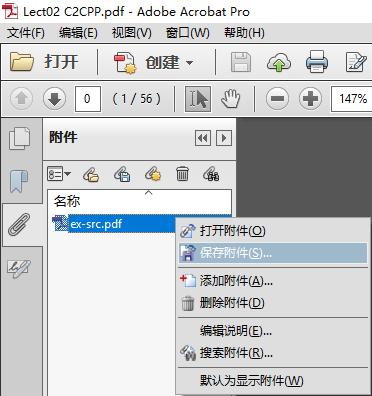
\includegraphics[height=0.35\textheight]{pdfattatchdownload01}\quad
    %或 \quad%
    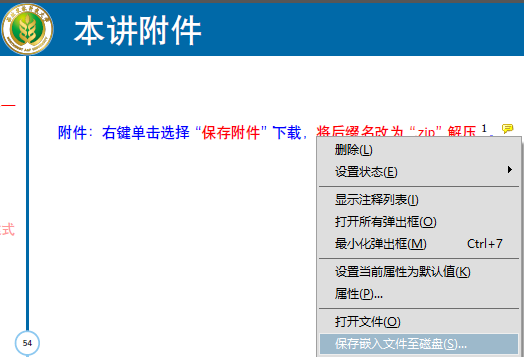
\includegraphics[height=0.35\textheight]{pdfattatchdownload02}\\[2ex]%
    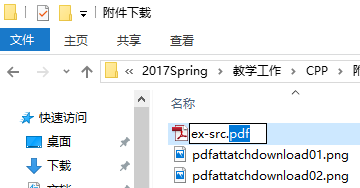
\includegraphics[height=0.255\textheight]{pdfattatchdownload03}\quad
    %$\Rightarrow$ \quad%
    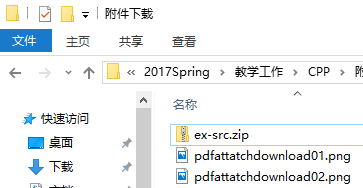
\includegraphics[height=0.255\textheight]{pdfattatchdownload04}%
  \end{center}   
\end{frame}

% \tiny
% \scriptsize
% \footnotesize
% \small
% \normalsize
% \large
% \Large
% \LARGE
% \huge
% \Huge


%%% Local Variables: 
%%% mode: latex
%%% TeX-master: "../main.tex"
%%% End: 
